\documentclass[12pt]{article}
\usepackage{amsmath}
\usepackage{graphicx}
\usepackage{enumerate}
\usepackage{setspace}
\usepackage{paralist}
\usepackage{caption}
\usepackage{subcaption}

\title{Project Report: Sparse RBM}
\author{Catherine Olsson}

\begin{document}

\maketitle

\section*{Overview}
In this project I demonstrate a reimplementation of the sparse Restricted Boltzmann Machine described in the first part of Lee et al. 2007. I demonstrate the following results:
\\
\begin{compactitem}
\item Constructed and trained a Restricted Boltzmann Machine (RBM) network on the MNIST dataset
\item Extended the RBM to implement the sparsity constraint described in Lee et al. (2007)
\item Computed the distribution of filter responses in the unmodified network as compared to the sparse network, and visualized the degree of sparsity in their responses, over images and over units
\item Demonstrated that the distribution of filter responses after training with the sparsity constraint is skewed such that each filter responds to fewer images on average, even in regularization regimes where the filters and samples do not look noticeably different from $\lambda=0$.
\item Inferred that the sparsity constraint I have implemented is operating differently than Lee et al; the behavior I see is that more and more filters successively drop out of any attempt to describe the data, unlike the smooth localized filters obtained by Lee et al.
\end{compactitem}

\section*{Background: sparsity and V1-like features in natural images}
I was first drawn to the topic of unsupervised feature-learning in shallow networks because of the implications for visual neuroscience. A variety of different objective functions trained on images have been shown to give rise to oriented Gabor-like filters, which share a resemblance with the sorts of filters found in primate visual area V1. Sparse coding (Olshausen and Field 1996) and Independent Components  Analysis (Bell and Sejnowski 1997) both represent unsupervised approaches which give rise to oriented gabor-like filters. Supervised approaches also give rise to these filters, including the sparse energy-based model approach of Ranzato et al. (2006), as well as the first layer of most modern Deep Neural Nets trained to perform image recognition on large datasets such as ImageNet (see Krizhevsky et al. 2012). All these approaches, except the supervised AlexNet-like approaches, include sparsity as a central constraint; some of these approaches do not give rise to Gabor-like filters if the sparsity constraint is not included. I wanted to explore the impact of sparsity on the nature and distribution of filters learned in response to images, and to gain more intuition about the practical aspects of working with and training neural networks on images.

\section*{Background: Restricted Boltzmann Machines (RBMs)}

Restricted Boltzmann Machines are a generative model architecture consisting of one layer of $m$ visible/observed input nodes ($\vec{v}$), fully connected to a layer of $n$ ``hidden'' nodes ($\vec{h}$). The weights between the visible and hidden nodes (along with the \texttt{vbias} and \texttt{hbias} terms) define an Energy function, which is a measure of consistency or compatibility between a given set of $\vec{v}$ values and a set of $\vec{h}$ values. Figure~\ref{rbmfan} shows a diagram of an RBM, from the \texttt{deeplearning.net} tutorial. The $\vec{h}$ values are binary; sampling a set of $\vec{h}$ values for a given $\vec{v}$ involves computing the output of the weights for each $h$, and then setting the binary outcome for each $h$ node binomially in proportion to the output of the weight computation.

Training an RBM is a process of adjusting the energy landscape to maximize the likelihood of the data. Training over a given batch involves two steps: one to ``push down'' on the observed training samples to make those configurations more likely, and the other to ``pull up'' on unobserved samples that the model nonetheless assigns high likelihood in order to raise the rest of the energy landscape (the second term is needed to prevent the landscape from collapsing or becoming degenerate). The first part - the ``positive phase'' of the gradient - can be computed directly using gradient descent on the training data or on a minibatch of examples, but the second part - the ``negative phase'' - needs to be estimated using a handful of generated examples, which are assigned high likelihood by the model but are not actually true training examples. Generating these ``negative particles'' involves running a chain of Gibbs sampling to produce generated examples.

\begin{figure}[h]
  \centering
  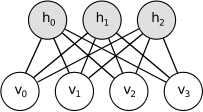
\includegraphics[width=0.3\textwidth]{rbmfan.png}
  \caption{Canonical depiction of the RBM architecture. The visible layer $v$ corresponds to pixels in image patches, and the hidden layer filters $h$ are each fully-connected to the input image layer}
  \label{rbmfan}
\end{figure}

\section*{Baseline: MNIST RBM}

As a baseline, before adding sparsity constraints, I trained the RBM on the MNIST dataset of handwritten digits (My RBM implementation and initial parameter choices owe their origins to the \texttt{deeplearning.net} tutorial code as a starting point). The subsection of MNIST I used for quick experimentation consisted of 10,000 greyscale images of size $28 \times 28$; I additionally ran a few longer tests with all 50,000 images in the dataset. I used 500 hidden units. I trained over a batch size of 20, with a learning rate of 0.1, for usually 10 or 15 training epochs. Lee et al. used 200 hidden units, but did not specify the learning rate, initialization, batch size, or other guidance about training. Additionally, Lee et al. used PCA whitening to project their data to 69 principal components before training, which I did not implement.

I attempted to train this network to perform well on the Van Hateren natural image dataset as well, but did not have enough time to select well-performing hyperparameters. The unsuccessful Van Hateren filters are shown in Figure~\ref{vanh1}. The main problem I encountered was that many of the filters refused to participate, and remained stuck at something close to their initialized starting point. For the remainder of the sparsity experiments, I decided to forge ahead with MNIST only.

\begin{figure}[h]
  \centering
  \begin{subfigure}{0.45\textwidth}
\includegraphics[width=\textwidth]{../figs/05_16_1509_mnist/filters_at_epoch_14.png}
  \caption{Successful attempt to train on MNIST}
  \label{mnist1}
  \end{subfigure}
  \begin{subfigure}{0.45\textwidth}
\includegraphics[width=\textwidth]{../figs/05_16_1606_vanhateren/filters_at_epoch_14.png}
  \caption{Abandoned attempt to train on image patches}
  \label{vanh1}
  \end{subfigure}
  \caption{Trained filters for regular RBM}
\end{figure}

\section*{Addition: Sparsity constraint}

After implementing the ordinary RBM, I added the sparsity constraint described in Lee et al. 2007. An important question when adding a sparsity constraint is to decide whether the purpose is, say, for a given image to activate only a few units, or for a given unit to activate for only certain images. In practice this may work out the same, but the two constraints take different forms. 

Lee et al. write their sparsity constraint as follows:

\begin{align*}
\lambda \Sigma_{j=1}^n |p - \frac{1}{m} \Sigma_{l=1}^m \mathbf{E} [h_j^{(l)} | \vec{v}^{(l)}] |
\end{align*}

I interpret this as, roughly, for each individual filter, to average all the expected $\vec{h}$ activations across all the images in the minibatch (where ``expected'' refers to the value computed before taking the binomial), and compute the absolute deviation from some low value $p$ for that filter, then to sum these deviations over all the filters. I interpret this to mean that Lee et al.'s update rule works out to encourage sparsity in the domain of ``how many images does each unit respond to''.  I chose $p=0$ because that was familiar from the sparsity formulations I had seen earlier in the class, but as I will speculate later in the report, this may have led my results to deviate from Lee et al's results.

\section*{Results: Filters and their response distributions, in default- versus sparse-RBM}

I trained the model four more times with different settings of lambda, and a smaller test size for faster iteration. The histograms below (Figure~\ref{sparse}) illustrate the distribution averaged two ways - over images (roughly capturing the distribution of unit firing rates) and over units (roughly capturing the distribution of how ``exciting'' the images are). 

One effect I noticed was that the distribution of filter responses between $\lambda=0$ and $\lambda=0.1$ was visibly skewed leftwards after training with the sparsity constraint, such that each filter responds to fewer images on average, even though to my bare eye the filters and samples do not look remarkably different.

I also noticed that for very high $\lambda$ values, the filters collapse and do not respond to anything, which is another reassuring sign that $\lambda$ is successfully enforcing low/sparse activations.

Finally I notice that the average over units does not change shape, although it does get lower, reffirming my belief that the sparsity constraint encourages each unit to fire to a sparse set of images images, but not encouraging each image to excite a sparse set of units.

\begin{figure}[h!]
    \centering
    \begin{subfigure}[b]{0.45\textwidth}
        \includegraphics[width=\textwidth]{../figs/fig_lambda0_avgoverims.png}
        \caption{Unit responses, avg over images}
    \end{subfigure}    
    \begin{subfigure}[b]{0.45\textwidth}
       
\includegraphics[width=\textwidth]{../figs/fig_lambda0_avgoverunits.png}
        \caption{Evoked responses, avg over units}
    \end{subfigure}    
    \caption{$\lambda=0$}

    \begin{subfigure}[b]{0.45\textwidth}
        \includegraphics[width=\textwidth]{../figs/fig_lambda0pt1_avgoverims.png}
        \caption{Unit responses, avg over images}
    \end{subfigure}    
    \begin{subfigure}[b]{0.45\textwidth}
       
\includegraphics[width=\textwidth]{../figs/fig_lambda0pt1_avgoverunits.png}
        \caption{Evoked responses, avg over units}
    \end{subfigure}    
    \caption{$\lambda=0.1$}

    \begin{subfigure}[b]{0.45\textwidth}
        \includegraphics[width=\textwidth]{../figs/fig_lambda0pt5_avgoverims.png}
        \caption{Unit responses, avg over images}
    \end{subfigure}    
    \begin{subfigure}[b]{0.45\textwidth}
       
\includegraphics[width=\textwidth]{../figs/fig_lambda0pt5_avgoverunits.png}
        \caption{Evoked responses, avg over units}
    \end{subfigure}    
    \caption{$\lambda=0.5$}

    \begin{subfigure}[b]{0.45\textwidth}
        \includegraphics[width=\textwidth]{../figs/fig_lambda10_avgoverims.png}
        \caption{Unit responses, avg over images}
    \end{subfigure}    
    \begin{subfigure}[b]{0.45\textwidth}
       
\includegraphics[width=\textwidth]{../figs/fig_lambda10_avgoverunits.png}
        \caption{Evoked responses, avg over units}
    \end{subfigure}    
    \caption{$\lambda=10$}

\end{figure}

\begin{figure}[h!]
    \begin{subfigure}[b]{0.45\textwidth}
\includegraphics[width=\textwidth]{../figs/05_17_123656_mnist/filters_at_epoch_9.png}
        \caption{$\lambda=0$}
    \end{subfigure}  
    \begin{subfigure}[b]{0.45\textwidth}
\includegraphics[width=\textwidth]{../figs/05_17_132506_mnist/filters_at_epoch_9.png}
        \caption{$\lambda=0.1$}
    \end{subfigure} 
\\
    \begin{subfigure}[b]{0.45\textwidth}
\includegraphics[width=\textwidth]{../figs/05_17_143833_mnist/filters_at_epoch_9.png}
        \caption{$\lambda=0.5$}
    \end{subfigure}  
    \begin{subfigure}[b]{0.45\textwidth}
\includegraphics[width=\textwidth]{../figs/05_17_140222_mnist/filters_at_epoch_9.png}
        \caption{$\lambda=10$}
    \end{subfigure} 
    \caption{Filters learned at varying sparsity levels}
    \label{sparse}
\end{figure}

\section*{Comparison with Lee et al. 2007}

By comparing the generated filters from my results with those generated by Lee et al. (2007) (see Figure~\ref{lee}), I can only infer that the sparsity constraint I have implemented is operating differently than Lee et al's. The behavior I see is that more and more filters successively drop out and revert to noise. This leads to a growing population of filters that do not respond to any of the input images, which is one way to obtain an overall sparse response in the filters. However, this behavior in the filters is unlike the smooth localized filters shown by Lee et al. There are several possibilities for why this discrepancy. My main hypothesis is that this relates to the $p$ parameter, and that driving neuron responses to a low but nonzero value would prevent collapse, instead of driving them towards zero. Another possibility is that the PCA whitening and dimensionality reduction, which I did not implement, plays an important role in the behavior of the sparsity constraint. Additionally, it is possible that the network behaves differently in different hyperparameter regimes (learning rates, amount of training data, patch size, etc.), and that these differences between my network and theirs are driving the differences in observed behavior. Finally, it is possible that I have misinterpreted the precise form of Lee et al.'s sparsity constraint, and have implemented it incorrectly

\begin{figure}[h!]
  \centering
  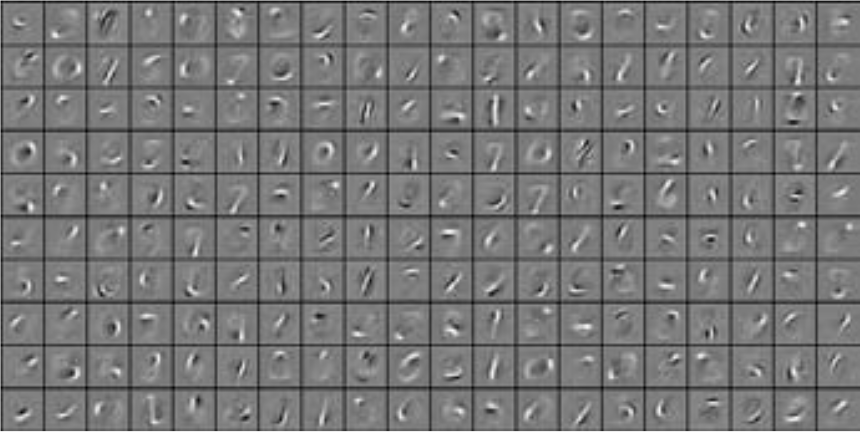
\includegraphics[width=0.7\textwidth]{lee_mnist_filters.png}
  \caption{Filters reported in Lee et al.}
  \label{lee}
\end{figure}

\section*{Resources}
Works to reference:
\\
\singlespace
\leftskip 0.5in
\parindent -0.5in


Bell, A. and Sejnowsky, T. (1997). The ``Independent Components'' of Natural Scenes are Edge Filters. \emph{Vision Research, 37}(23), 3327-3338.

Krizhevsky, A., Sutskever, I., and Hinton, G. Classification with Deep Convolutional Neural Networks. (2012). \emph{Advances in Neural Information Processing Systems}(25).

Lee, H., Ekanadham, C., and Ng, A. (2007). Sparse Deep Belief Net Model for Visual Area V2. \emph{Advances in Neural Information Processing Systems}(20).

Ranzato, M., Poultney, C., Chopra, S., and LeCun, Y. (2006). Efficient Learning of Sparse Representations with an Energy-Based Model. \emph{Advances in Neural Information Processing Systems}(19).

van Hateren, J., and Ruderman. D. (1998). Independent component analysis of natural image sequences yields spatio-temporal filters similar to simple cells in primary visual cortex. \emph{Proc. R. Soc. Lond. B}(265), 2315-2320.

Hoyer, P., and Hyvärinen A. (2002). A multi-layer sparse coding network
learns contour coding from natural images. \emph{Vision Research, 42}(12), 1593-1605.

Hyvarinen, A., Gutmann, P., and Hoyer, P. (2005). Statistical model of natural stimuli predicts edge-like pooling of spatial frequency channels in V2. \emph{BMC Neuroscience, 6}(12).

Olshausen, B. and Field, J. (1996). Emergence of simple-cell receptive field properties by learning a sparse code for natural images. \emph{Nature}(381), 607-609


\end{document}
